\setcounter{MaxMatrixCols}{20}
\chapter{Stratégie}
\label{cp:strategie}

Même si le démineur est un jeu simple, une IA parfaite n'aurait pas 100\% de victoire. En effet, c'est un jeu de probabilités, et il existe donc des situations dans lesquelles la possibilité de trouver un bombe dans chaque
case non-révélée est équiprobable. Dans ce cas, l'IA doit faire un choix aléatoire.
\newline
Notre stratégie sera donc de calculer la probabilité de chaque case non-révélée de contenir une bombe, et de choisir une des cases avec la plus faible probabilité.

\section{Preliminaires}

Dans toute la suite de ce chapitre, on considère une grille de démineur de taille $n \times m$ avec $b$ bombes, et on note $G$ la grille, $G_{i,j}$ la case à la ligne $i$ et la colonne $j$.
\newline
$G_{i,j} = -1$ si la case n'est pas révélée, $G_{i,j} = k$ si la case est révélée et contient $k$ bombes autour d'elle.

\section{Algorithme naïf}

Calculer la probabilité de chaque case non-révélée de contenir une bombe est une tâche complexe : une information à un bout de la grille peut influencer une case à l'autre bout.
\newline
Intuitivement, on commence par essayer de faire du dénombrement : on calcule toutes les combinaisons possibles de bombes, et ne garde que les combinaisons valides, et on compte le nombre de fois où chaque case est une bombe.

\subsection{Dénombrement}

On construit un algorithme qui, pour une grille $G$ donnée calcule toutes les combinaisons possibles de bombes, et ne garde que les combinaisons valides.
\newline
Il y a deux difficultés majeures à résoudre :
\begin{itemize}
    \item Comment valider une combinaison ?
    \item Comment éviter de tester des combinaisons qui sont évidemment invalides ?
\end{itemize}

Pour répondre à ces problèmes, on introduit une idée simple, mais qui nous sera utile dans la suite : on va grouper des cases ensemble.
\newline
On définit un groupe comme un ensemble de cases non-révélées. 
\newline
Dans cet algorithme, pour chaque case révélée, on crée un groupe avec les cases adjacentes.
\newline
On peut alors, pour chaque combinaison de 2 groupes, trouver l'intersection de ces derniers, et poser une condition sur les cases de cette intersection.

\subsection{Pseudo-code}

\begin{longlisting}
    \begin{minted}{text}
        Fonction Probabilite
        Parametres :
            n en entier, m en entier
            G en matrice d'entiers de taille n x m
        Declarations :
            groupes en liste de listes de couples d'entiers
            intersections en liste de listes de couples d'entiers
            P en matrice d'entiers
            combinaisons en liste de listes de couples d'entiers
            combinaisons_valides en entier
        Sortie :
            P en matrice de reels de taille n x m
        Debut
            P = matrice de 0 de taille n x m
    
            groupes = liste des groupes des cases révélées

            intersections = liste des intersections de chaque combinaison de 2 groupes

            combinaisons = []
            Pour k allant de 1 a |groupes| faire
                Ajouter a combinaisons une liste de toutes les combinaisons possibles de G[i][j] bombes dans les cases de groupes[k]
            FinPour

            combinaisons_valides = 0
            Pour chaque element du produit cartesien de combinaisons faire
                Pour chaque intersection dans intersections faire
                    Si l'intersection contient plus de bombes que le nombre de bombes autour de chaque case dans l'intersection alors
                        Continuer
                    FinSi
                FinPour

                Pour chaque case dans l'element faire
                    P[case] += 1
                FinPour
                combinaisons_valides += 1
            FinPour

            Pour i allant de 1 a n faire
                Pour j allant de 1 a m faire
                    Si G[i,j] = -1 alors
                        P[i,j] /= combinaisons_valides
                    FinSi
                FinPour
            FinPour

            Retourner P
        Fin
    \end{minted}
    \caption{Pseudo-code de l'algorithme naif de calcul de probabilité}
    \label{listing:algo-naif}
\end{longlisting}

\subsection{Complexité}

La complexité de cet algorithme est très élevée, car il faut calculer le produit cartésien de toutes les combinaisons possibles de bombes : la complexité est exponentielle en le nombre de cases non-révélées.
Cet algorithme est donc inutilisable pour des grilles de taille moyenne.
\newline
Si on veut calculer les probabilités de chaque case, il va falloir radicalement optimiser cette stratégie.

\section{Algorithme optimisé}

Pour optimiser cet algorithme, on va représenter notre problème sous une forme différente. 
\newline
On commence par définir un graphe $G'$, où chaque sommet est une case, et où il y a une arête entre deux cases si elles sont adjacentes.
On construit alors la matrice A de taille $n*m \times n*m$ telle que $A_{(i, j), (i', j')} = 1$ si ${(i, j)}$ et ${(i', j')}$ sont adjacents, et $0$ sinon. C'est la matrice d'adjacence de $G'$.
\newline
On remarque alors que l'ont peut très facilement retrouver la matrice $G$ complète (c'est à dire avec toutes les cases révélées) à partir de $A$ et de la position des bombes.
\newline
\newline
Notons $B$ la colonne de taille $n*m$ telle que $B_i = 1$ si la case $i$ contient une bombe, et $0$ sinon.
De même, soit $v$ la colonne de taille $n*m$ telle que $v_i = G_{i,j}$ si la case $i$ est révélée, et $-1$ sinon.
\newline
\newline
On a alors la relation suivante :
\[
A \cdot B = v
\]
\newline
Cette relation est un système linéaire, que l'on peut résoudre pour trouver toutes les colonnes $B$ qui satisfassent $v$ (c'est à dire toutes les positions possible de bombes qui respectent les cases révélées).
Nous pouvons alors calculer la probabilité de chaque case non-révélée de contenir une bombe.

\subsection{Optimizations}

Représenter le problème sous forme de système linéaire ne change pas la complexité de la résolution du problème, résoudre le système entier revient à la même complexité que l'algorithme naïf.
Mais cette représentation nous permet de faire des optimisations qui vont nous permettre de réduire la complexité de l'algorithme.
\newline
\newline
Prenons un exemple simple :

\begin{figure}[!htpb]
    \centering
    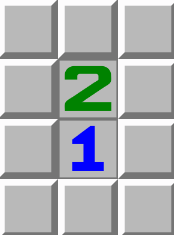
\includegraphics[width=0.2\linewidth]{Figures/exemple-board.png}
    \caption[Exemple de grille]{Exemple de grille.}
    \label{fig:exemple-board}
\end{figure}

On obtient les matrices suivantes : (A est symétrique, on ne montre que la moitié de la matrice)
\[
    A = \begin{pmatrix}
        0 & 1 & 0 & 1 & 1 & 0 & 0 & 0 & 0 & 0 & 0 & 0 \\
          & 0 & 1 & 1 & 1 & 1 & 0 & 0 & 0 & 0 & 0 & 0 \\
          &   & 0 & 0 & 1 & 1 & 0 & 0 & 0 & 0 & 0 & 0 \\
          &   &   & 0 & 1 & 0 & 1 & 1 & 0 & 0 & 0 & 0 \\
          &   &   &   & 0 & 1 & 1 & 1 & 1 & 0 & 0 & 0 \\
          &   &   &   &   & 0 & 0 & 1 & 1 & 0 & 0 & 0 \\
          &   &   &   &   &   & 0 & 1 & 0 & 1 & 1 & 0 \\
          &   &   &   &   &   &   & 0 & 1 & 1 & 1 & 1 \\
          &   &   &   &   &   &   &   & 0 & 0 & 1 & 1 \\
          &   &   &   &   &   &   &   &   & 0 & 1 & 0 \\
          &   &   &   &   &   &   &   &   &   & 0 & 1 \\
          &   &   &   &   &   &   &   &   &   &   & 0 \\
    \end{pmatrix}
    \hspace{1cm}
    v = \begin{bmatrix} -1 \\-1 \\-1 \\-1 \\2 \\-1 \\ -1 \\1 \\-1 \\-1 \\-1 \\-1 \\ \end{bmatrix}
\]

On commence par ne garder que les lignes de $A$ et de $v$ qui correspondent à des cases révélées.
On peut enlever ces lignes car on ne connait pas la valeur de ces cases dans $v$, les utiliser pour résoudre le système ne nous apporterait aucune information.
\newline
\newline
On enleve aussi les colonnes de $A$ qui correspondent à des cases révélées, car il ne peut y avoir de bombes dans ces cases.
\newline
On obtient alors :
\[
    A = \begin{pmatrix}
        1 & 1 & 1 & 1 & 1 & 1 & 1 & 0 & 0 & 0 \\
        0 & 0 & 0 & 1 & 1 & 1 & 1 & 1 & 1 & 1 \\
    \end{pmatrix}
    \hspace{1cm}
    v = \begin{bmatrix} 2 \\1 \\ \end{bmatrix}
\]

On remarque alors que plusieurs colonnes de $A$ sont identiques, on va donc les regrouper.
Ce regroupement n'est pas intuitif, on est en fait en train de grouper les cases qui sont influencées par les mêmes cases révélées.
Ce dernier est possible car on sait que chaque case d'un groupe à la même probabilité de contenir une bombe.
\newline
Dans notre exemple, on obtient ces groupes :

\begin{figure}[!htpb]
    \centering
    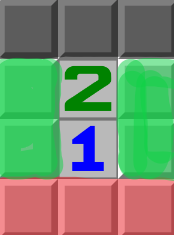
\includegraphics[width=0.2\linewidth]{Figures/groups-on-board.png}
    \caption[Grille avec les groupes en couleur]{Grille avec les groupes en couleur.}
    \label{fig:groups-on-board}
\end{figure}

On groupe alors ces colonnes :
\[
    A = \begin{pmatrix}
        1 & 1 & 0 \\
        0 & 1 & 1 \\
    \end{pmatrix}
    \hspace{1cm}
    v = \begin{bmatrix} 2 \\1 \\ \end{bmatrix}
\]

Trouver un solution à ce système revient à distribuer des bombes dans les groupes. On connait le nombre de cases dans chaque groupe, on peut alors facilement calculer la probabilité de chaque case de contenir une bombe.
\newline
\newline
On utilise l'algorithme de Gauss-Jordan pour réduire la matrice $A$ en forme échelonnée réduite :
\[
    A = \begin{pmatrix}
        1 & 0 & -1 \\
        0 & 1 & 1 \\
    \end{pmatrix}
    \hspace{1cm}
    v = \begin{bmatrix} 1 \\1 \\ \end{bmatrix}
\]

Dans un cas classique, ce système aurait une infinité de solutions, mais dans notre cas, on peut mettre des bornes sur les variables (le nombres de bombes par groupe).
Initialement, ces bornes sont $[0, |groupe|]$, mais on peut les réduire grâce au système $A|v$.
\newline
On cherche alors les variables libres, c'est à dire les colonnes de $A$ qui ne sont pas des pivots. Les solutions sont alors les combinaisons de ces variables qui respectent les bornes.
\newpage
Dans notre exemple, on a une seule variable libre, la dernière colonne de $A$. Les solutions sont alors :
\[
    \begin{bmatrix} 2 \\0 \\1 \\ \end{bmatrix}
    \hspace{1cm}
    \begin{bmatrix} 1 \\1 \\0 \\ \end{bmatrix}
\]

Retrouver la probabilité de chaque case revient à trouver la probabilité de chaque solution. On obtient alors :
\[
    \mathbb{P}(\text{Solutions}_k) = \prod_{i=1}^{|\text{Groupes}|} \binom{|\text{Groupe}_i|}{\text{Solution}_i}
\]
\[
    \mathbb{P}(\text{Groupes}_k) = \sum_{i=1}^{|\text{Solutions}|} \frac{\mathbb{P}(\text{Solutions}_i) \times \text{Solution}_k}{|\text{Groupes}_k|}
\]

Finallement, toute les cases d'un groupe ont la probabilité de ce groupe de contenir une bombe.